%%%%%%%%%%%%%%%%%%%%%%% file template.tex %%%%%%%%%%%%%%%%%%%%%%%%%
%
% This is a template file for Web of Conferences Journal
%
% Copy it to a new file with a new name and use it as the basis
% for your article
%
%%%%%%%%%%%%%%%%%%%%%%%%%% EDP Science %%%%%%%%%%%%%%%%%%%%%%%%%%%%
%
%%%\documentclass[option]{webofc}
%%% "twocolumn" for typesetting an article in two columns format (default one column)
%
\documentclass{webofc}
\usepackage[varg]{txfonts}   % Web of Conferences font
\usepackage{subfigure}
%
% Put here some packages required or/and some personnal commands
%
%
\begin{document}
%
\title{Factory Monitoring for the 21st Century}
%
% subtitle is optionnal
%
%%%\subtitle{Do you have a subtitle?\\ If so, write it here}

\author{\firstname{Jeffrey} \lastname{Dost}\inst{1}\fnsep\thanks{\email{jdost@ucsd.edu}} \and
        \firstname{Edgar} \lastname{Fajardo}\inst{1}\fnsep\thanks{\email{emfajard@ucsd.edu}} \and
        \firstname{Brian} \lastname{Bockelman}\inst{2} \and
        \firstname{Leonardo} \lastname{Hern\'andez-Cano}\inst{3} \and
        \firstname{Caitlin} \lastname{Hung}\inst{1} \and
        \firstname{Naveen} \lastname{Kashyap}\inst{1} \and
        \firstname{Frank} \lastname{W\"urthwein}\inst{1} \and
        \firstname{Marian} \lastname{Zvada}\inst{2}
        % etc.
}

\institute{University of California, San Diego, 9500 Gilman Dr, La Jolla, CA 92093, USA 
\and
           University of Nebraska-Lincoln, 1400 R Street, Lincoln, NE 68588, USA
\and
           National Autonomous University of Mexico, Av Universidad 3000, Copilco Universidad, Coyoac\'an, Ciudad de M\'exico, Distrito Federal 04510, Mexico
          }

\abstract{%
  A key aspect of pilot-based grid operations are the GlideinWMS pilot factories. A proper and efficient use of any central block in the grid infrastructure for operations is inevitable, and GlideinWMS factories are no exception. The monitoring package for the GlideinWMS factory was originally developed when the factories were serving a couple of VOs and tens of sites. Today with the factories serving tens of VOs and hundreds of sites around the globe an update of the monitoring is due. Moreover with the new availability of industry open source storage and graphing packages an opportunity remains open. This work presents the changes made to the factory monitoring to leverage different technologies: Elasticsearch, RabbitMQ, Grafana, and InfluxDB to provide a centralized view of the status and work of several GlideinWMS factories located in different continents around the globe.
}
%
\maketitle
%
\section{Introduction}
\label{intro}
The OSG Glidein Factory \cite{FactoryOps} is an integral service for CMS and OSG \cite{osg}. The factory operations team depends on monitoring information for a variety of tasks such as ensuring the health of the service, making sure pilots are being submitted to sites the end users are requesting, and ensuring the pilots run at sites without issue. The GlideinWMS software \cite{GlideinWMSSoft} comes with standard web-based monitoring pages built in. When the OSG Glidein factory first went live, it was a single instance, and served about four scientific communities or Virtual Organizations(VO). Pilots were all configured to run only in single core mode. Over time, as more VOs joined OSG and adapted GlideinWMS, the scale of the OSG Factory grew to the point where more than one instance was required to run in parallel to serve the load. In addition to scaling in size, eventually CMS and other VOs began experimenting with multicore pilots. This is just one example of new resource types the factory software had to adapt to. Over the lifetime of the OSG Factory as a service, these evolutionary changes were needed to keep up with the demands of the users, but at the same time disrupted the monitoring, and code had to be adjusted to keep up with the changes.

Fundamental changes such as providing multicore pilot metrics were eventually added, but the updates were limited to the case where pilots requested a fixed number of cores, and the user jobs either still ran in single core mode, or a single user job would take over all cores of a given pilot. When more sophisticated modes of multicore were adapted such as partitionable slots -- which allowed users to dynamically select a subset of cores of a given pilot -- again, the monitoring needed to be changed to reflect this new mode of operation.

In addition to proper accounting of core usage, as more factories were spun up, it became evident to the operations team that having individual web pages for each factory would not be sufficient to give a global picture of the OSG Factory as a whole. A long standing request has been made to the GlideinWMS developers to provide an aggregate monitoring solution that combined usage of all factories. However in practice, other more urgent feature requests kept the global monitoring request at a lower priority, and it was never implemented. Over the years it was becoming apparent that a better development workflow was needed to keep up with factory monitoring needs. In 2017 the Open Science Grid agreed to take ownership of the factory monitoring. This would allow the GlideinWMS developers to focus on non-monitoring related development, they would merely need to provide a way to export the raw metrics in a parsable format. At the same time, dedicated staff at UCSD and UNL could work with the Factory Operations team and ensure monitoring needs are met as disruptive changes occur in the evolution of the Glidein factory.

\section{Architecture}
\label{arch}
The new factory monitoring architecture is iteratively being improved and revised, but this section will focus on two implementations, and will be referred to as Version 1 (Sect.~\ref{arch-pre}), and Version 2 (Sect.~\ref{arch-post}), which is the current implementation. Version 1 was presented as a poster at CHEP 2018. Significant improvements have been made since, so the discussion on Version 2 will explain what was changed, the reasons for the changes, and how the current implementation has improved as a result. Before getting into the new architecture, first the original GlideinWMS factory monitoring will be discussed in the next section.

\subsection{GlideinWMS built-in monitoring}
\label{arch-orig}
The GlideinWMS built-in factory monitoring is based around the RRDtool database \cite{rrdtool}, which is a round robin database intended to store time based series for fixed amounts of time. RRDs are schema based, so unfortunately if any metrics are added or removed to the series, all of the existing RRDs must be updated to account for the change. The factory provides a web server that hosts plots over time of statistics of pilots running at sites all over the globe. For each site queue a corresponding RRD database has to be maintained in the backend. The plots are generated by parsing the RRDs using JavaScript libraries. All of the web pages were created from the ground up, mostly by students. Because of this, it is difficult to make changes to the existing pages. Metrics along with their views, such as layout, colors, and line types are all hardcoded values in the web code, they cannot be customized without committing changes to the GlideinWMS codebase. Also, as stated previously, each factory instance has its own web server containing monitoring pages describing itself only. One factory monitor does not contain information about other factories.

\subsection{New monitoring: Version 1}
\label{arch-pre}
The first step toward decoupling factory monitoring from particular instances was to split the data store and user interface from the factory code. For the data store, InfluxDB \cite{influxdb} was initially chosen because it was created to hold time series data. Its advantage over RRD is that it is schema-less, so the data series don't need to be defined in advance; metrics can be added or removed metrics arbitrarily without committing to a particular layout. On the user interace end, Grafana was chosen because it is web-based like the previous monitoring, it supports InfluxDB natively, and its ability to create views including graphs and tables is very flexible and customizable. Both InfluxDB and Grafana were installed on a new monitoring host at UCSD separate from the factories.

The next step was to devise a method to push the data from the factories into InfluxDB. The GlideinWMS factory code already published some pilot statistics in a parsable XML file called \verb"schedd_status.xml". This XML file is published on the factory web servers and is periodically updated along side the RRD files. It contains current statistics such as counts of running, idle, and held at various site queues. In order to leverage this, a Python script was devised that would periodically run as a cron job on each factory called \verb"factory_monitor.py". The \verb"factory_monitor.py" script reads in the current values from \verb"schedd_status.xml" and updates the relevant InfluxDB databases on the monitoring host over HTTP. This functionality was abstracted into a library named the messenger module. The idea is that a specific messenger module can be written to push data to InfluxDB, but then later other messenger modules can be written that to push to other database types, and they would all be envoked the same way.

The above solution works well for plotting the queued pilot statuses over time, however the old GlideinWMS monitoring also contained plots based on completion statistics that were directly pushed to the RRD files without being exported to a status XML file. To reproduce these missing plots, a patch was written to also export the missing completed stats into a new file, which later became a feature of GlideinWMS. These statistics contain information such as how much walltime the pilots spent running, counts of pilots passing or failing validation, the number of user jobs ran inside the pilots, and other runtime characteristics of the user jobs. These metrics are exported in a file called \verb"completed_data.json". The JSON format was chosen for the missing file because it has become a more commonly used file format for sending data to modern database solutions such as InfluxDB and Elasticsearch \cite{elasticsearch}. A request has been made to the GlideinWMS team to also convert \verb"schedd_status.xml" to a JSON file. If JSON can replace XML as the native format for what already exists and for exporting future metrics, extra conversion steps from XML to JSON would be no longer needed whenever monitoring information is parsed from the state files.

\subsection{New monitoring: Version 2}
\label{arch-post}
The Version 1 setup was enough to provide a proof of concept prototype, and it was used to successfully decouple the factory monitoring from the factory code. However, further work had to be done to take the new monitoring a step further and provide a way for data to be pushed to more than one backend. The Grid Accounting Collector (GRACC) \cite{gracc} is the official monitoring Elasticsearch instance for OSG. It is a natural place to also back up all factory statistics. Planning to also feed the GRACC Elasticsearch revealed limitations in the current setup. In order to publish data to it, one must first coordinate with UNL to push data to a RabbitMQ \cite{rabbitmq} instance maintained by Nebraska. The UNL operations team handles the path from RabbitMQ into the GRACC Elasticsearch backend. The primary reason UNL uses a RabbitMQ message bus is for system resilience. It decouples the updates from the Elasticsearch database. That way if the database goes down for maintenance, or is replaced, data updates won't be lost. The requirement for updating the new factory monitoring setup was to modify the \verb"factory_monitor.py" script to also be able to push the data to the Nebraska RabbitMQ instance.

To prototype the changes needed to interface with Elasticseach via RabbitMQ, a test Elasticsearch instance was installed on the Grafana monitoring host at UCSD. A test RabbitMQ instance was set up on a different test machine also hosted at UCSD. Once the new Elasticsearch test infrastructure was ready, the limitation of our architecture became apparent. In order to better streamline the development pipeline and achieve quicker turnaround time for code updates, the decision was made to move the script off of the factories, and have it installed on a separate test machine at UCSD. This machine happened to be the same sharing the UCSD test RabbitMQ instance, but that is a temporary implementation detail. The reason why this still works is because the respective \verb"schedd_status.xml" and \verb"completed_data.json" files that publish the raw data on the production factories are also accessible via HTTP from any external host.

Besides moving the \verb"factory_monitor.py" script out of the factories and onto its own host, the code was updated to handle multiple factory sources, and updated with the ability to export the data to multiple database destinations. The script now simply loops over a list of factories, and parses the \verb"completed_data.json" and \verb"schedd_status.xml" files for each. The list of factories is configurable. In order to support multiple destinations, a messenger module was simply added that understands how to push the monitoring data to a RabbitMQ host. This module is invoked along with the already existing InfluxDB messenger module from the Version 1 implementation, and currently also sends the monitoring metrics to the UCSD test RabbitMQ instance. Work is still being done to reuse the RabbitMQ messenger module and also feed the Nebraska RabbitMQ instance, and ultimately to send the data to the OSG GRACC system.

\section{Results}
\label{results}
The fundamental test to ensure our new monitoring system is a viable candidate to replace the built-in GlideinWMS monitoring is to try and replicate the most used plots. Figure~\ref{running} and Figure~\ref{idle} show before and after snapshots comparing the built-in monitoring with new plots created in Grafana. The data source of these plots is the \verb"schedd_status.xml" file. Similarly, Figure~\ref{walltime} and Figure~\ref{validation} show the before and after for plots derived from the \verb"completed_data.json" source. Aside from slight differences in color choices more appropriate to the default dark theme of Grafana, for the purposes of daily factory operations, these plots are one to one replicas.

An important fundamental difference in the way the new plots are generated vs the old monitoring is that the rules used to generate them are completely decoupled from any code. The user interface in Grafana lets one add and modify plots arbitrarily on the fly. Conversely the built-in GlideinWMS plot definitions are hard-coded in the web monitor JavaScript. Arbitrary changes are not possible without pull requests to the GlideinWMS developers, and then waiting for the patches to be released in the next version of GlideinWMS rpms.

Another result worth noting is that graphs have been successfully replicated using both the InfluxDB and Elasticsearch data store backends. Grafana has built in support for both, so it is trivial to point it to either database type. The query languages are different, but Grafana allows one to write the queries required based on the configured backend, and generate visualizations with either. The test Grafana instance is currently configured to interface with both backends, so separate dashboards contain the respective plots generated from Influx and Elasticsearch. The important implication here is that implementation is not stuck using a particular data store, the new monitoring system is flexible to handle a variety of options.

\begin{figure}
\centering
\begin{minipage}[t]{.45\textwidth}
\subfigure[built-in]{\label{running:old}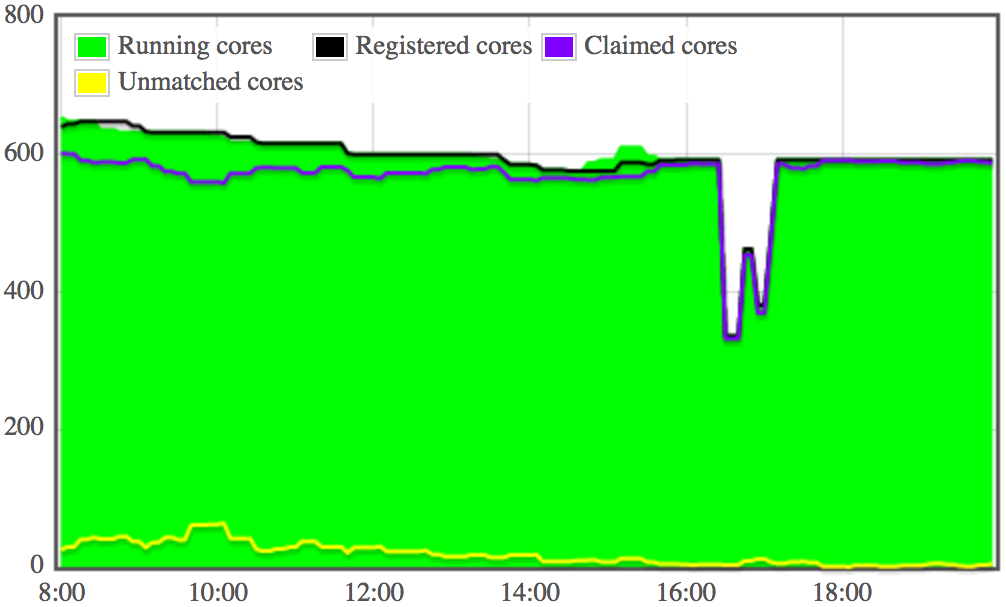
\includegraphics[width=\textwidth, height=1.05in]{images/running_gwms2.png}}
\subfigure[Grafana]{\label{running:new}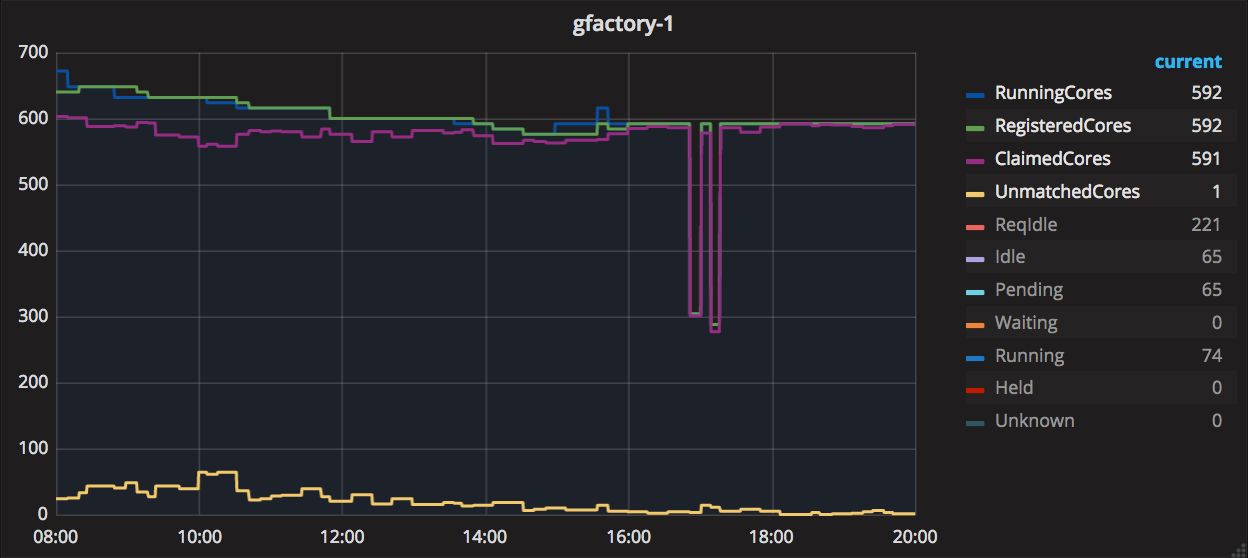
\includegraphics[width=\textwidth, height=1.05in]{images/running_grafana2.png}}
\caption{Comparison of running pilots at a particular compute element from built-in GlideinWMS vs new Grafana monitoring}
\label{running}
\end{minipage}\hspace{.1in}
\begin{minipage}[t]{.45\textwidth}
\subfigure[built-in]{\label{idle:old}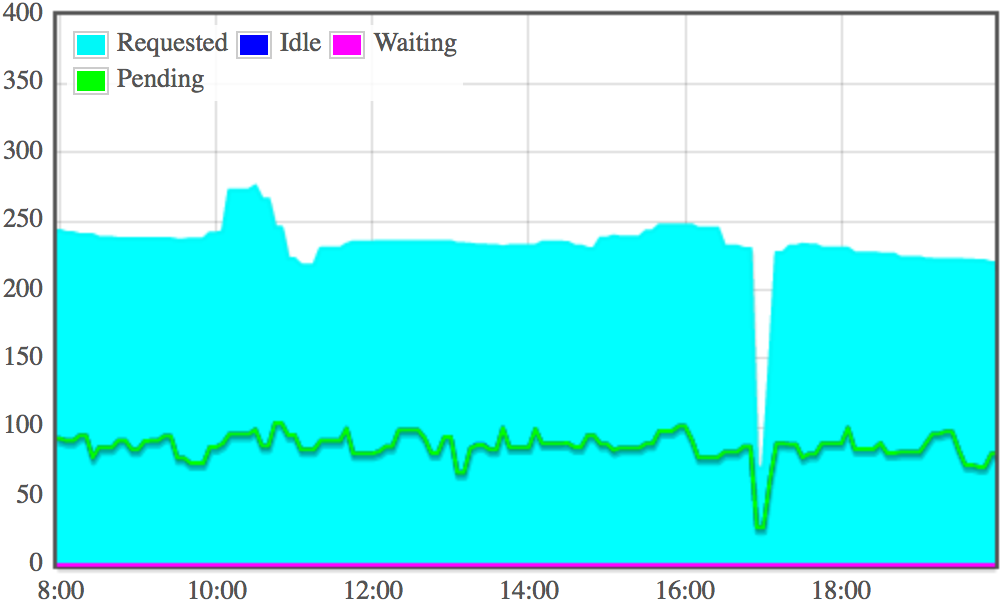
\includegraphics[width=\textwidth, height=1.05in]{images/idle_gwms2.png}}
\subfigure[Grafana]{\label{idle:new}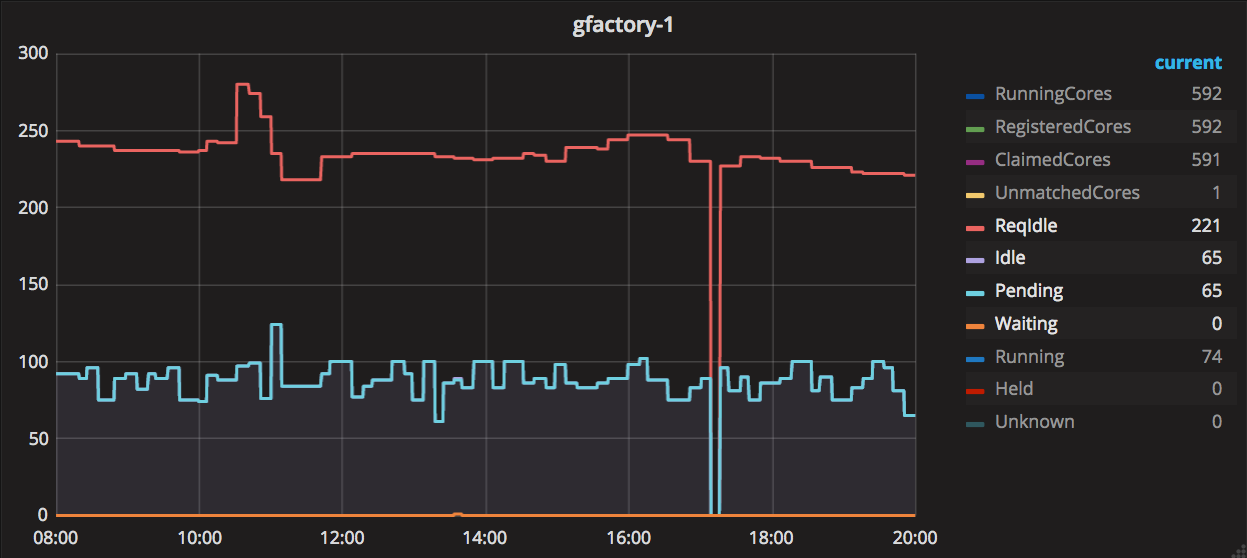
\includegraphics[width=\textwidth, height=1.05in]{images/idle_grafana2.png}}
\caption{Comparison of idle pilots at a particular compute element from built-in GlideinWMS vs new Grafana monitoring}
\label{idle}
\end{minipage}
\end{figure}

\begin{figure}
\centering
\begin{minipage}[t]{.45\textwidth}
\subfigure[built-in]{\label{walltime:old}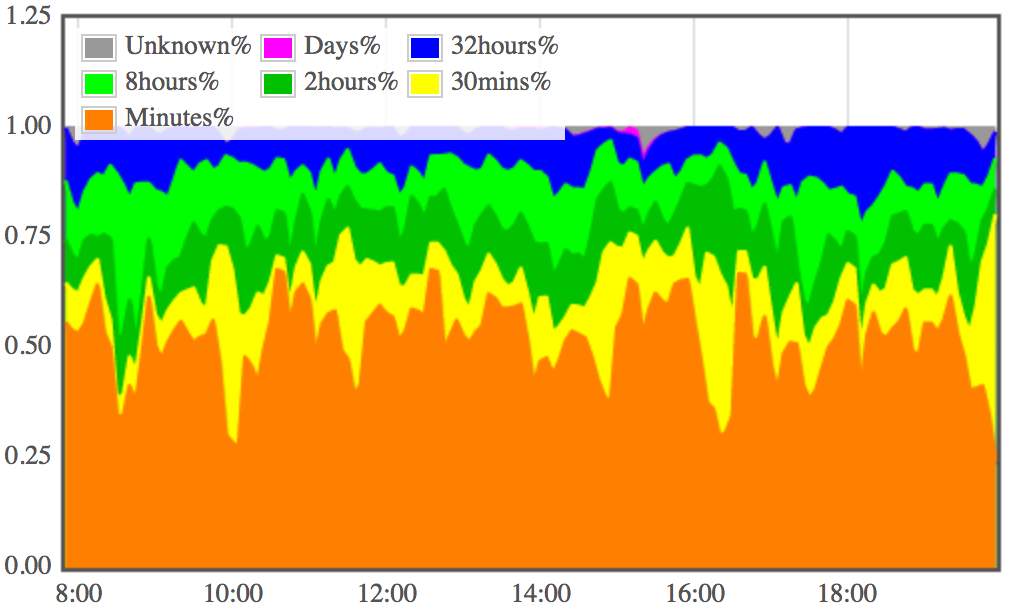
\includegraphics[width=\textwidth, height=1.05in]{images/walltime_gwms2.png}}
\subfigure[Grafana]{\label{walltime:new}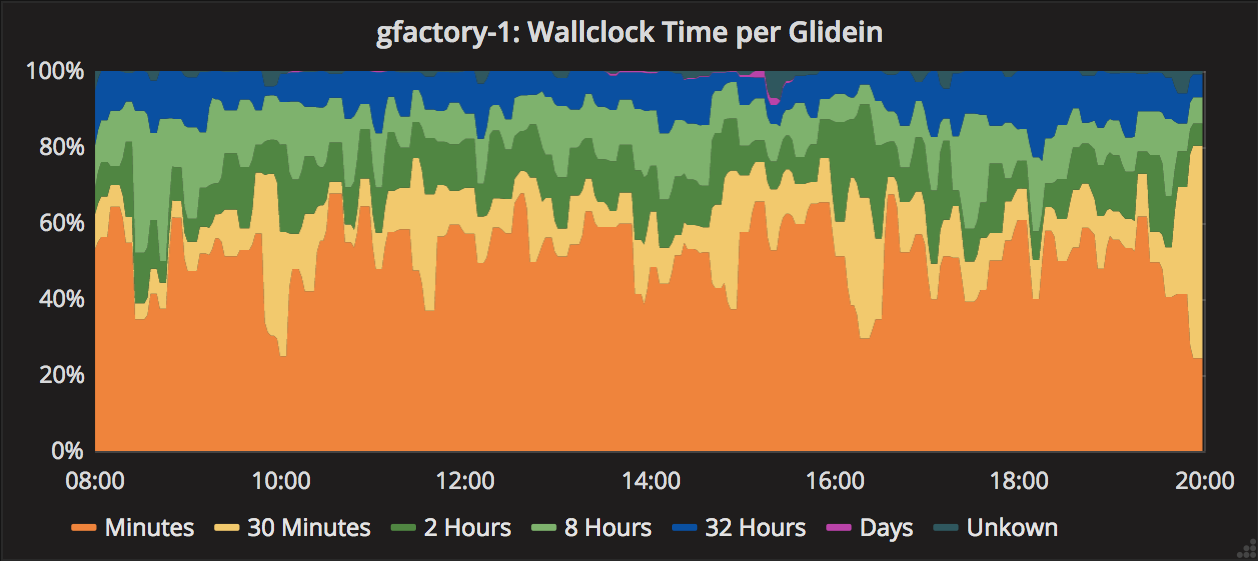
\includegraphics[width=\textwidth, height=1.05in]{images/walltime_grafana2.png}}
\caption{Comparison of pilot walltime at a particular factory from built-in GlideinWMS vs new Grafana monitoring}
\label{walltime}
\end{minipage}\hspace{.1in}
\begin{minipage}[t]{.45\textwidth}
\subfigure[built-in]{\label{validation:old}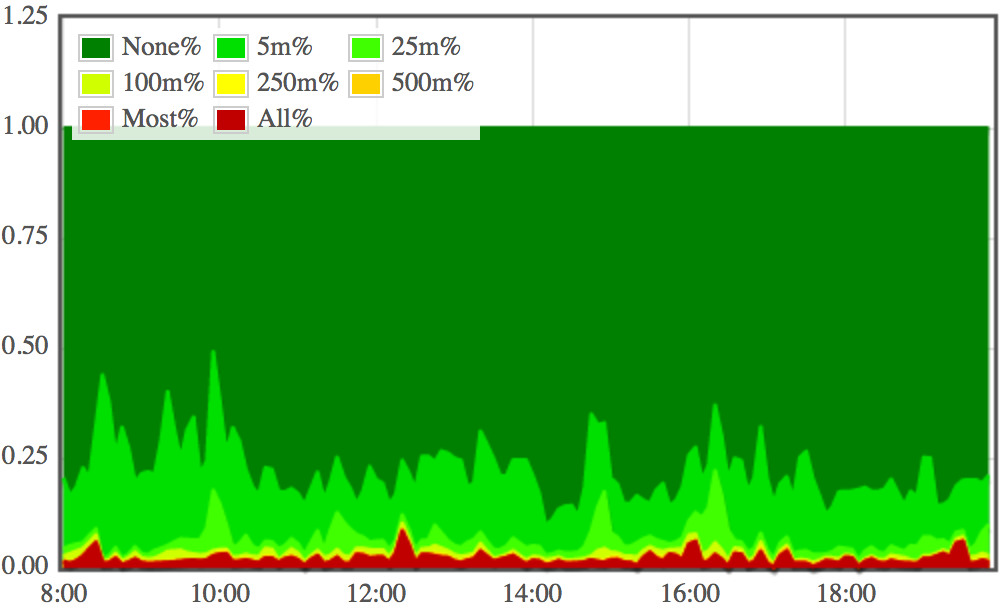
\includegraphics[width=\textwidth, height=1.05in]{images/validation_gwms2.png}}
\subfigure[Grafana]{\label{validation:new}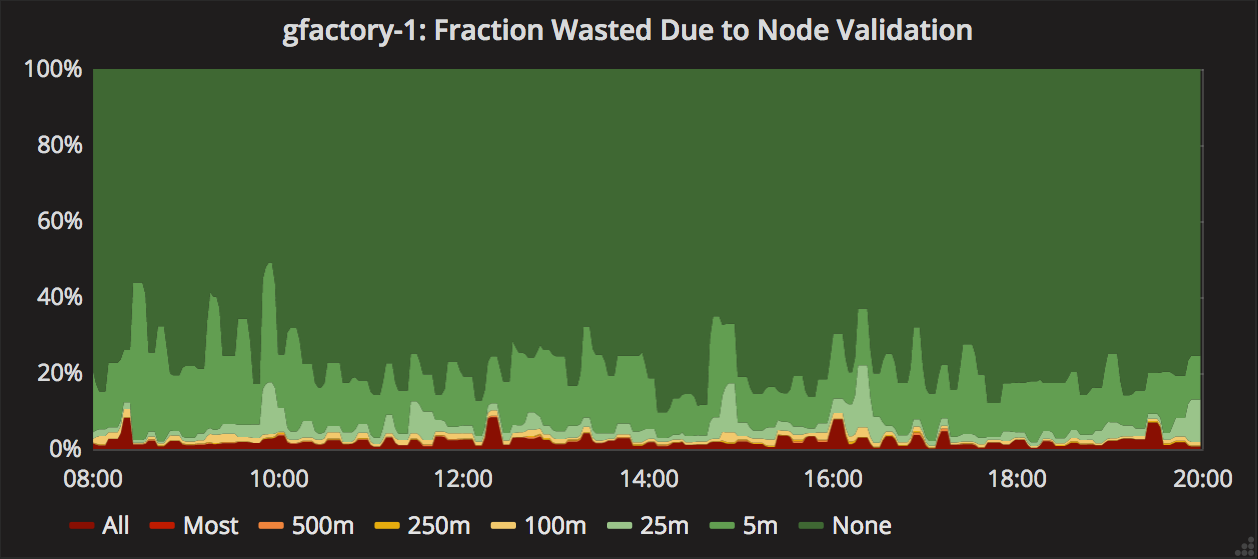
\includegraphics[width=\textwidth, height=1.05in]{images/validation_grafana2.png}}
\caption{Comparison of pilot validation failures at a particular factory from built-in GlideinWMS vs new Grafana monitoring}
\label{validation}
\end{minipage}
\end{figure}

\section{Conclusions}
\label{conclusions}
The new factory monitoring builds on and improves the original GlideinWMS factory monitoring in a few fundamental ways: it decouples the publishing of raw data from the monitor database backends, pulls the implementation out of the factory code and onto a separate host allowing aggregation of data from multiple factories, and modularizes the code to take advantage of a variety of latest standard monitoring tools used in industry and throughout the HEP computing community.

\bibliography{references}

\end{document}

% end of file template.tex

<div id='footer'><table width='100%'><tr><td class='right'><a href='http://fusioninventory.org/'><span class='copyright'>FusionInventory 9.1+1.0 | copyleft <img src='/glpi/plugins/fusioninventory/pics/copyleft.png'/>  2010-2016 by FusionInventory Team</span></a></td></tr></table></div>